% !TeX spellcheck = en_US
% !TeX root = ../build/l2-scaling-solutions.tex
% !TeX TXS-program:compile = txs:///xelatex/[--shell-escape]


\section{Introduction to Layer 2}


L2 layers are be established on top of the L1 infrastructure. These L2 layers have the authority to dictate their own state management procedure. For example, a payment system with simple transactions, a token transfer system or a EVM execution capability. Moreover, L2 layers have the autonomy to define their utilization of the underlying L1 architecture, encompassing two pivotal aspects: the L1 execution layer's usage and the interaction with the data shards (when available). Regarding the current situation of data sharding, L1 data shards specification is still under develop (the \textbf{EIP 4484} is currently on the ``review stage"). For this reason, currently, all the scaling solutions use only the availability of the execution layer.

For the sake of illustration, let's consider an instance of an L2 layer denoted by $L2_x$. In this scenario, \textbf{$L2_x$ transactions} form the foundational operations within $L2_x$. These transactions shape the state progression of $L2_x$. Figure \ref{fig:l2-state-sequence} illustrates how the different $L2_x$ states change with the execution of new sets of transactions.

\begin{figure}[h]
\centering
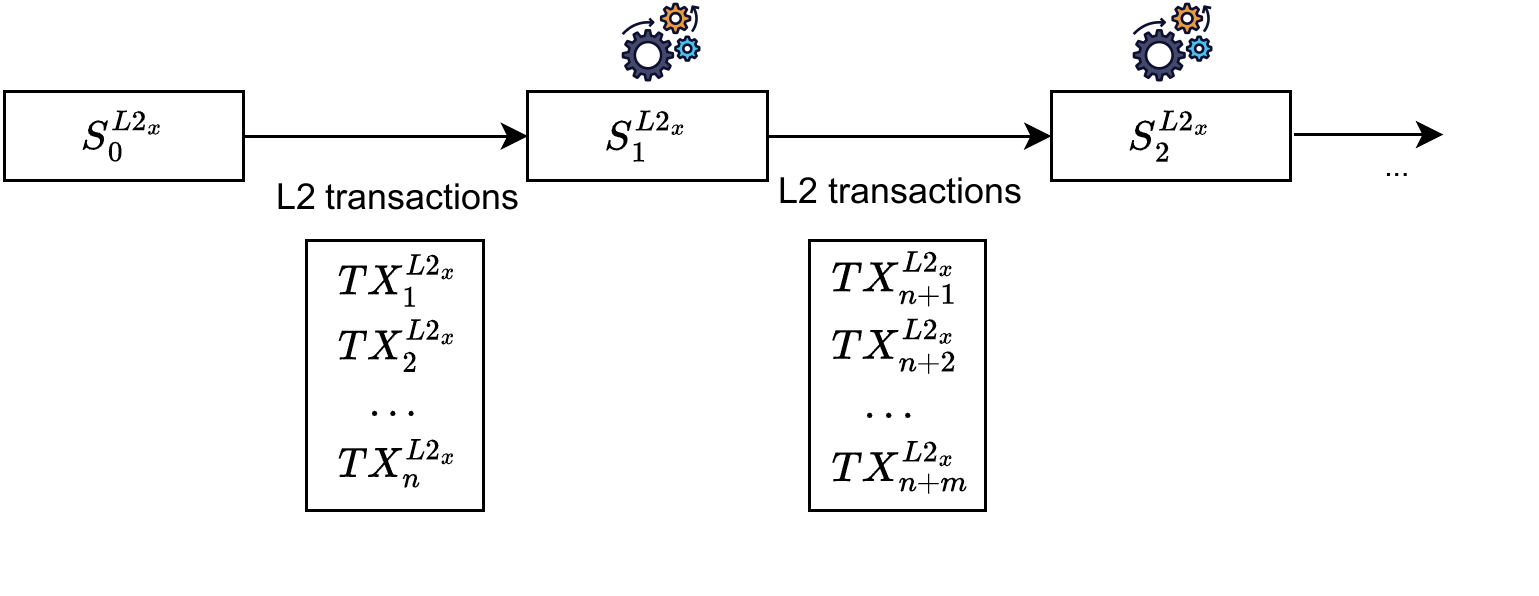
\includegraphics[width=.75\columnwidth]{\trainingsectiondir/figures/l2-state.drawio}
\caption{L2 State evolution via the execution of sets of L2 transactions.}
\label{fig:l2-state-sequence}
\end{figure}

Within this context, several questions naturally emerge:

\begin{enumerate}[(a)]

\item \textbf{Transaction Dissemination}: \textit{How do users initiate and direct $L2_x$ transactions, and who are the receivers of these transactions?}

\item \textbf{Transaction Data Availability}: \textit{Is there a mechanism in place to make L2 transactions publicly accessible, and if so, what methods are employed to achieve this transparency within the $L2_x$ ecosystem?}

\item \textbf{Transaction Processing and State Verification}: \textit{Who bears the responsibility for processing L2 transactions, what methodologies govern this processing, and when is it publicly affirmed that a new state has been accurately computed within $L2_x$?}

\item \textbf{Supported Application Complexity}: \textit{What types of applications find their home within $L2_x$? Does this layer cater primarily to straightforward, basic processing, or does it have the capacity to facilitate more intricate operations like EVM-like opcodes?}

\end{enumerate}

While it's important to note that the answers may not be unique due to the existence of different approaches (each one having its pros and cons), the following points will provide responses to all of the questions posed.

\subsection{Transaction Reception}

In the context of transaction origination and reception, there exists various communication paradigms that may dictate how L2 transactions are disseminated:

\begin{itemize}

\item \textbf{Unicast}: This dissemination mode involves the creation of a one-way communication channel with a centralized receiver (See Figure \ref{fig:unicast-diss}). In this scenario, L2 transactions are directed towards a specific centralized recipient.

\begin{figure}[h]
\centering
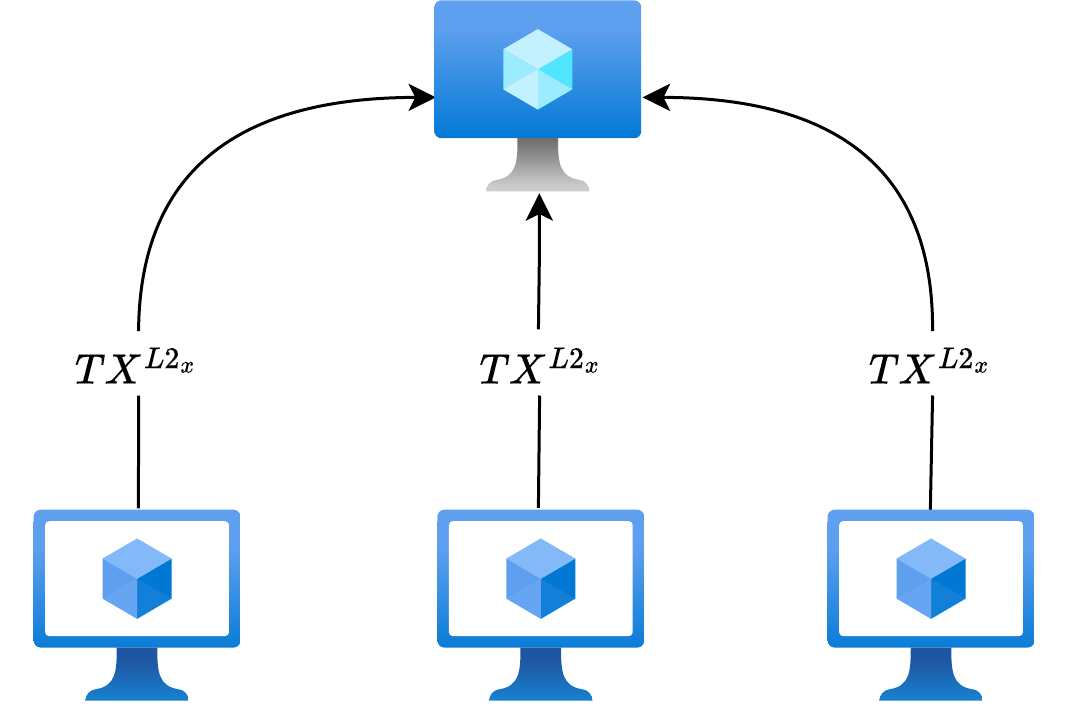
\includegraphics[width=.3\columnwidth]{\trainingsectiondir/figures/unicast.drawio}
\caption{Schema of Unicast communication.}
\label{fig:unicast-diss}
\end{figure}

\item \textbf{Peer-to-peer}: In a peer-to-peer network (See Figure \ref{fig:p2p-diss}), every participant, in a decentralized fashion, receives and processes L2 transactions. This approach emphasizes decentralized, distributed communication, ensuring that all network participants have access to the transactions.

\begin{figure}[h]
\centering
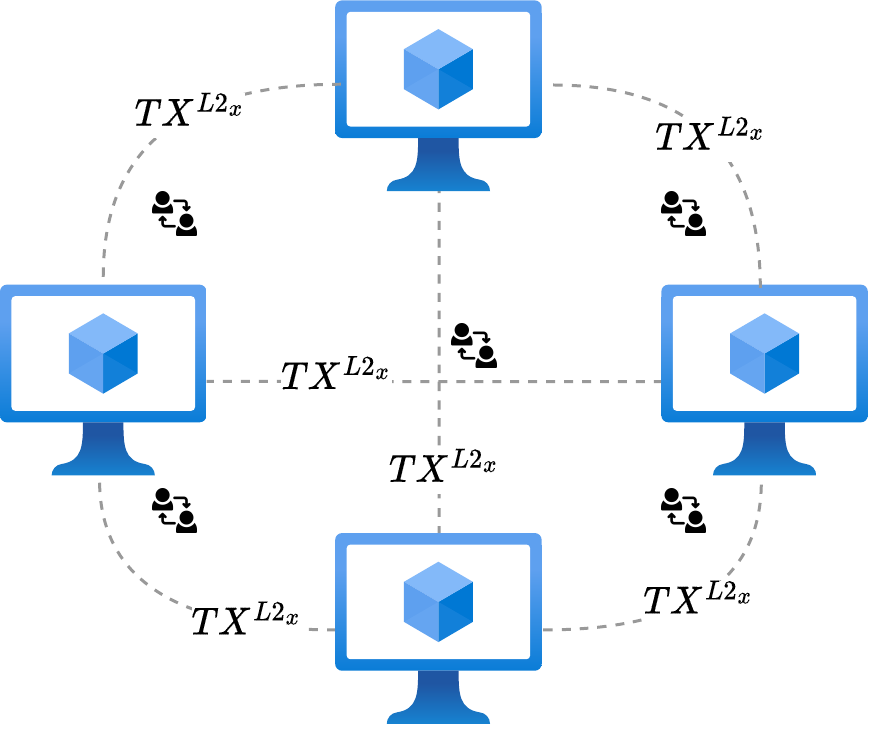
\includegraphics[width=.3\columnwidth]{\trainingsectiondir/figures/peer-to-peer.drawio}
\caption{Schema of Peer-to-Peer communication.}
\label{fig:p2p-diss}
\end{figure}

\item \textbf{Smart Contract}: Another approach to dissemination is through smart contracts within the L1 execution layer (See Figure \ref{fig:sc-diss}). These smart contracts operate in a decentralized manner and play a role in managing and processing L2 transactions.

\begin{figure}[h]
\centering
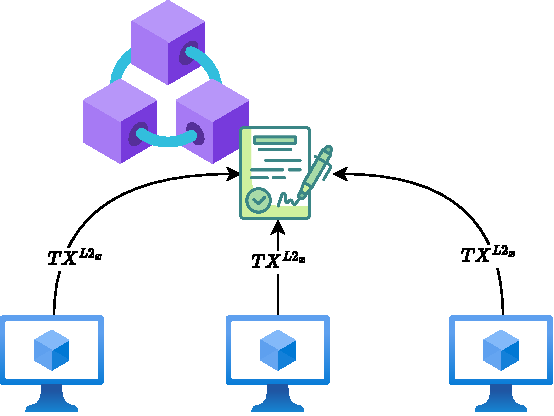
\includegraphics[width=.3\columnwidth]{\trainingsectiondir/figures/sc-l2-tx.drawio}
\caption{Schema of Smart Contract like communication.}
\label{fig:sc-diss}
\end{figure}

\end{itemize}

\subsection{Transaction Data Availability}

To achieve L2 data availability in Ethereum, currently, we can proceed in two
ways:

\begin{itemize}

\item \textbf{Validium Approach}: In this approach (Figure \ref{fig:validium}), L1 transactions only contain a cryptographic summary (a hash) of the corresponding L2 transactions. This design does not allow a user to retrieve L2 data from another layer, such as the L1 top layer. Instead, L2 data is overseen and managed by a consortium of trusted entities known as \textit{data managers}. Hence, users should rely on data managers to access L2 data.

\begin{figure}[h!]
\centering
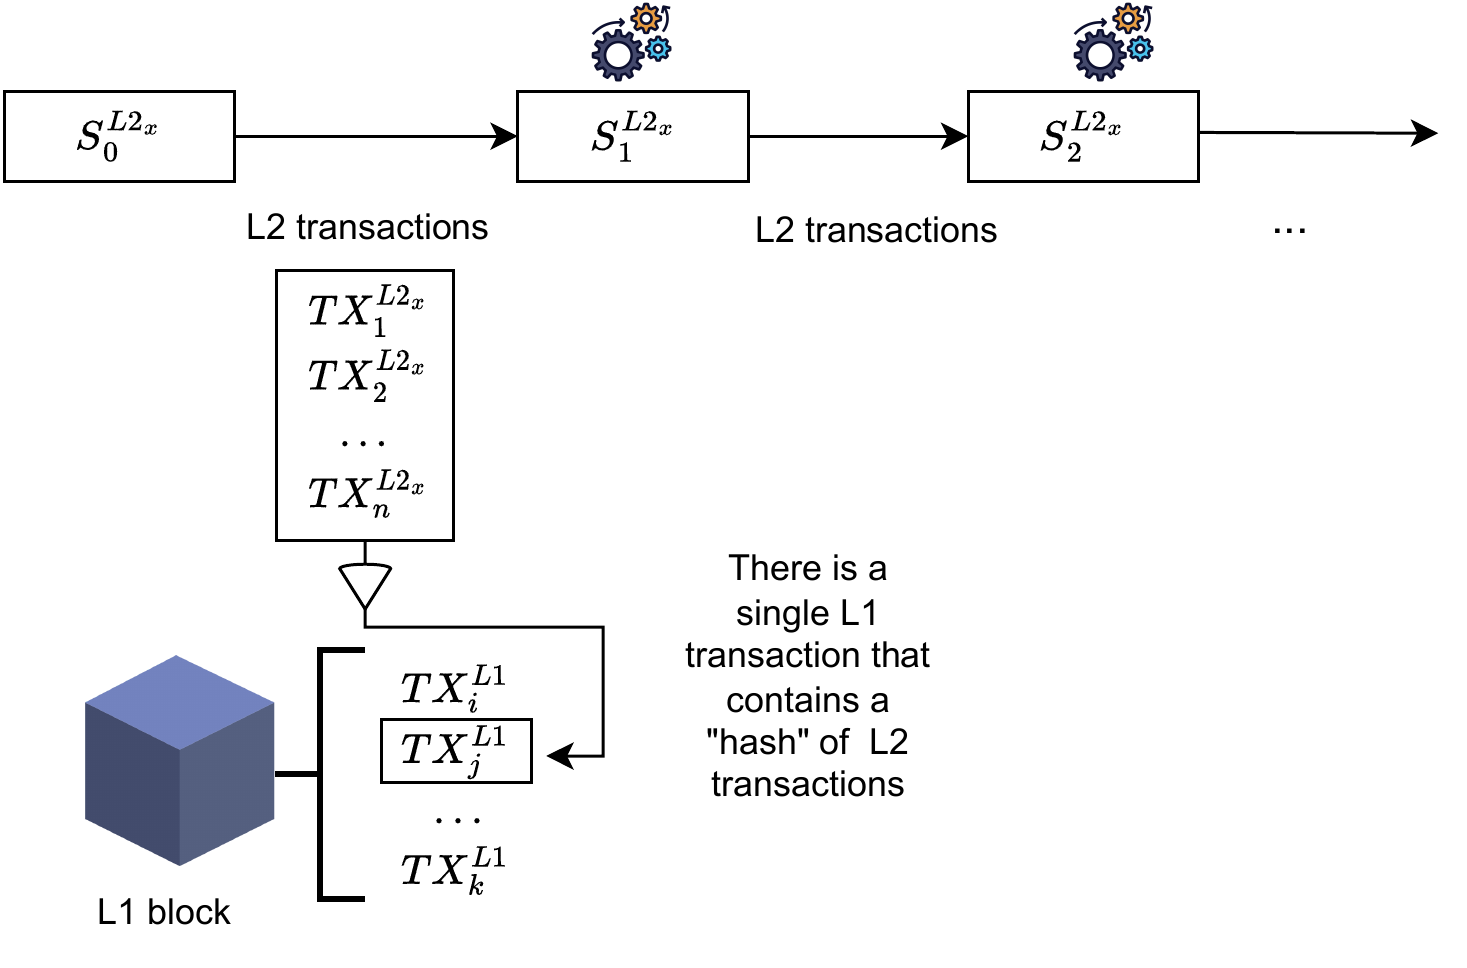
\includegraphics[width=.65\columnwidth]{\trainingsectiondir/figures/l2-validium.drawio}
\caption{Data Availability with the Validium Approach.}
\label{fig:validium}
\end{figure}



\item \textbf{Rollup Approach}: Alternatively, a \textbf{rollup} mechanism can be employed. This method involves writing L2 data to the public L1 execution layer, making the posted data publicly accessible to all participants on the blockchain network (See Figure \ref{fig:rollup}). In this case, to provide data availability, we use a single L1 transaction that contains a batch of L2 transactions. This method is called a rollup, because we \textit{roll up} a bunch of L2 transactions in a single L1 transaction.

\begin{figure}[h!]
\centering
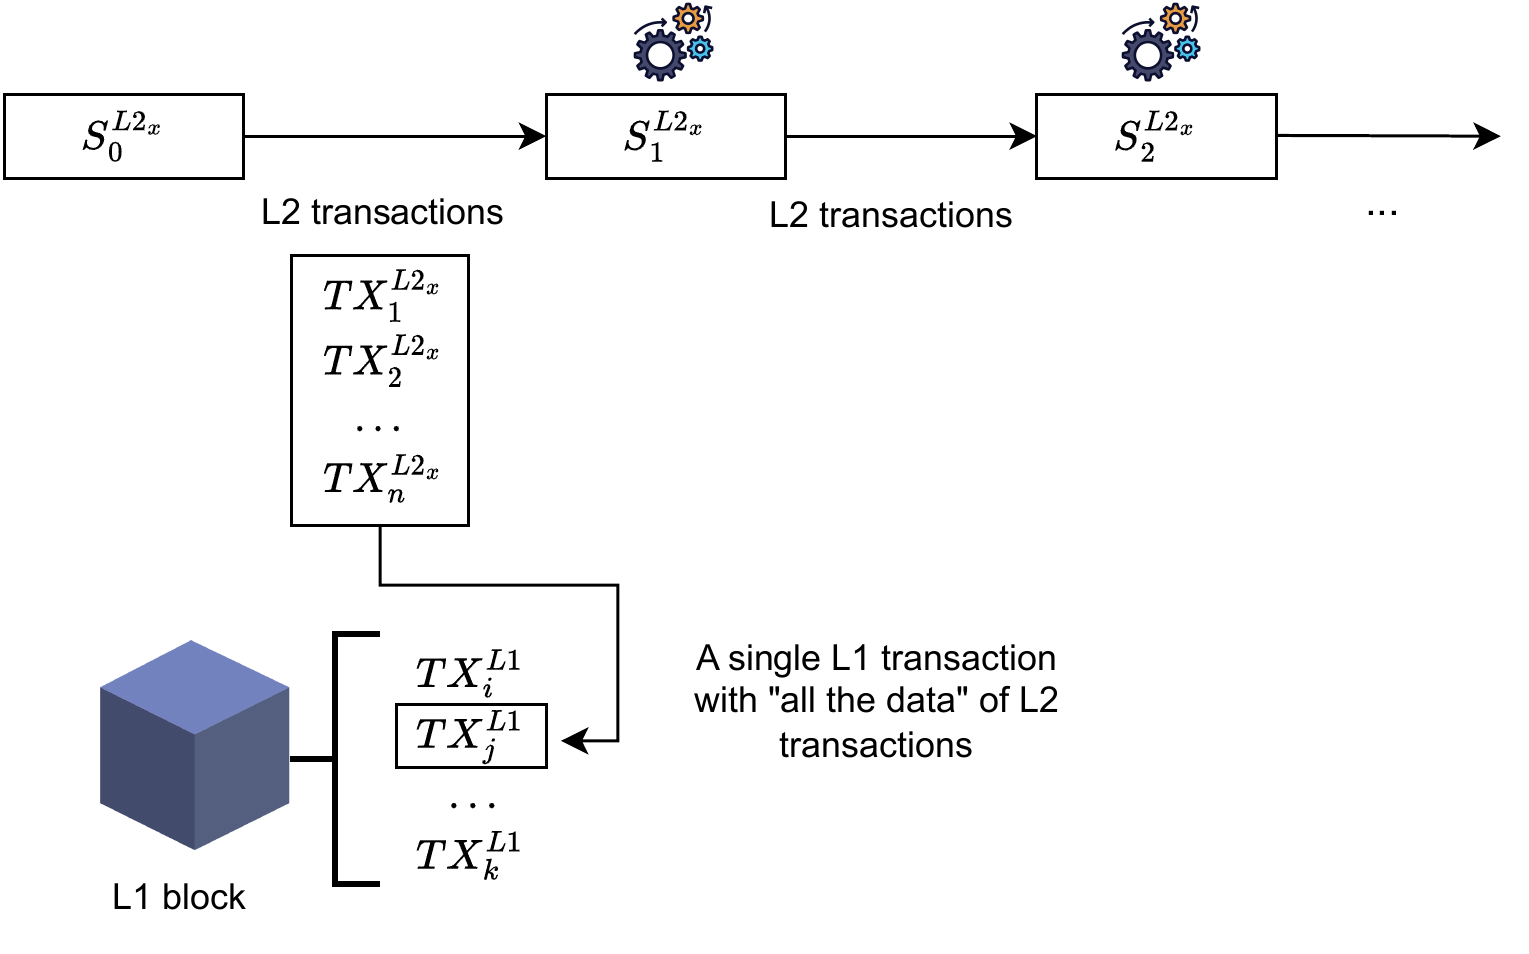
\includegraphics[width=.65\columnwidth]{\trainingsectiondir/figures/l2-rollup.drawio}
\caption{Data Availability with the Rollup Approach.}
\label{fig:rollup}
\end{figure}

\end{itemize}


\subsection{Transaction Processing and State Verification}

In the context of computing the subsequent L2 state $S^{L2_x}_{i+1}$ based on a set of $L2_x$ transactions and the present state $S^{L2_x}_i$, several distinct approaches can be employed. These approaches encompass:

\begin{itemize}

\item \textbf{Centralized Execution}: One approach involves centralized execution (See Figure \ref{fig:centralized-execution}), where a central entity is responsible for processing L2 transactions and computing the new L2 state. In this approach, the process of finalizing state computation occurs quite rapidly, typically taking only a matter of ``seconds or minutes". However, this approach introduces a significant challenge: \textit{how external entities can effectively raise disputes with the L2 operator regarding the accuracy and correctness of an L2 state computation}.

\begin{figure}[h!]
\centering
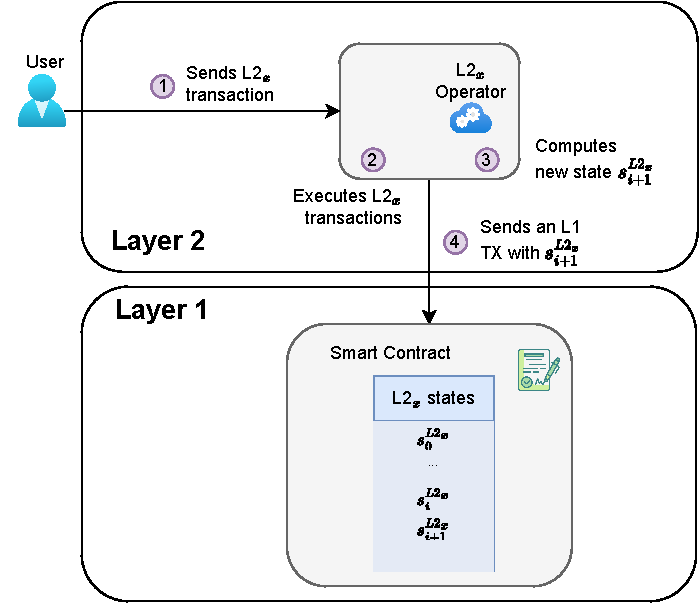
\includegraphics[width=.75\columnwidth]{\trainingsectiondir/figures/l2-centralized-design.drawio}
\caption{Centralized Execution Schema.}
\label{fig:centralized-execution}
\end{figure}

\item \textbf{Optimistic Execution}: An alternative method is optimistic execution, characterized by a trust-first approach. In this scenario, L2 transactions are executed \textit{optimistically}, that is, assuming they are valid, and only in cases of disputes the transactions are rigorously verified. An Optimistic L2 provides a decentralized execution mechanism that allows disputing the correctness of the L2 state computation. With this approach, there is a (large) period of time to allow anybody to send a \textbf{fraud proof} (See Figure \ref{fig:optimistic-execution}), proving that the state was wrongly computed (for example, a double spending transaction). Under the this model, if those who execute L2 transactions (referred to as the \textbf{optimistic executors}) correctly perform their duties, they stand to earn ETH as a reward for their correct execution. However, in cases where an optimistic executor fails to execute transactions correctly, they face a penalty in the form of slashing and the actor that provides the fraud proof (referred to as the \textbf{state checker}) is rewarded for that task. This approach aims to strike a balance between efficiency and security.

\begin{figure}[h!]
\centering
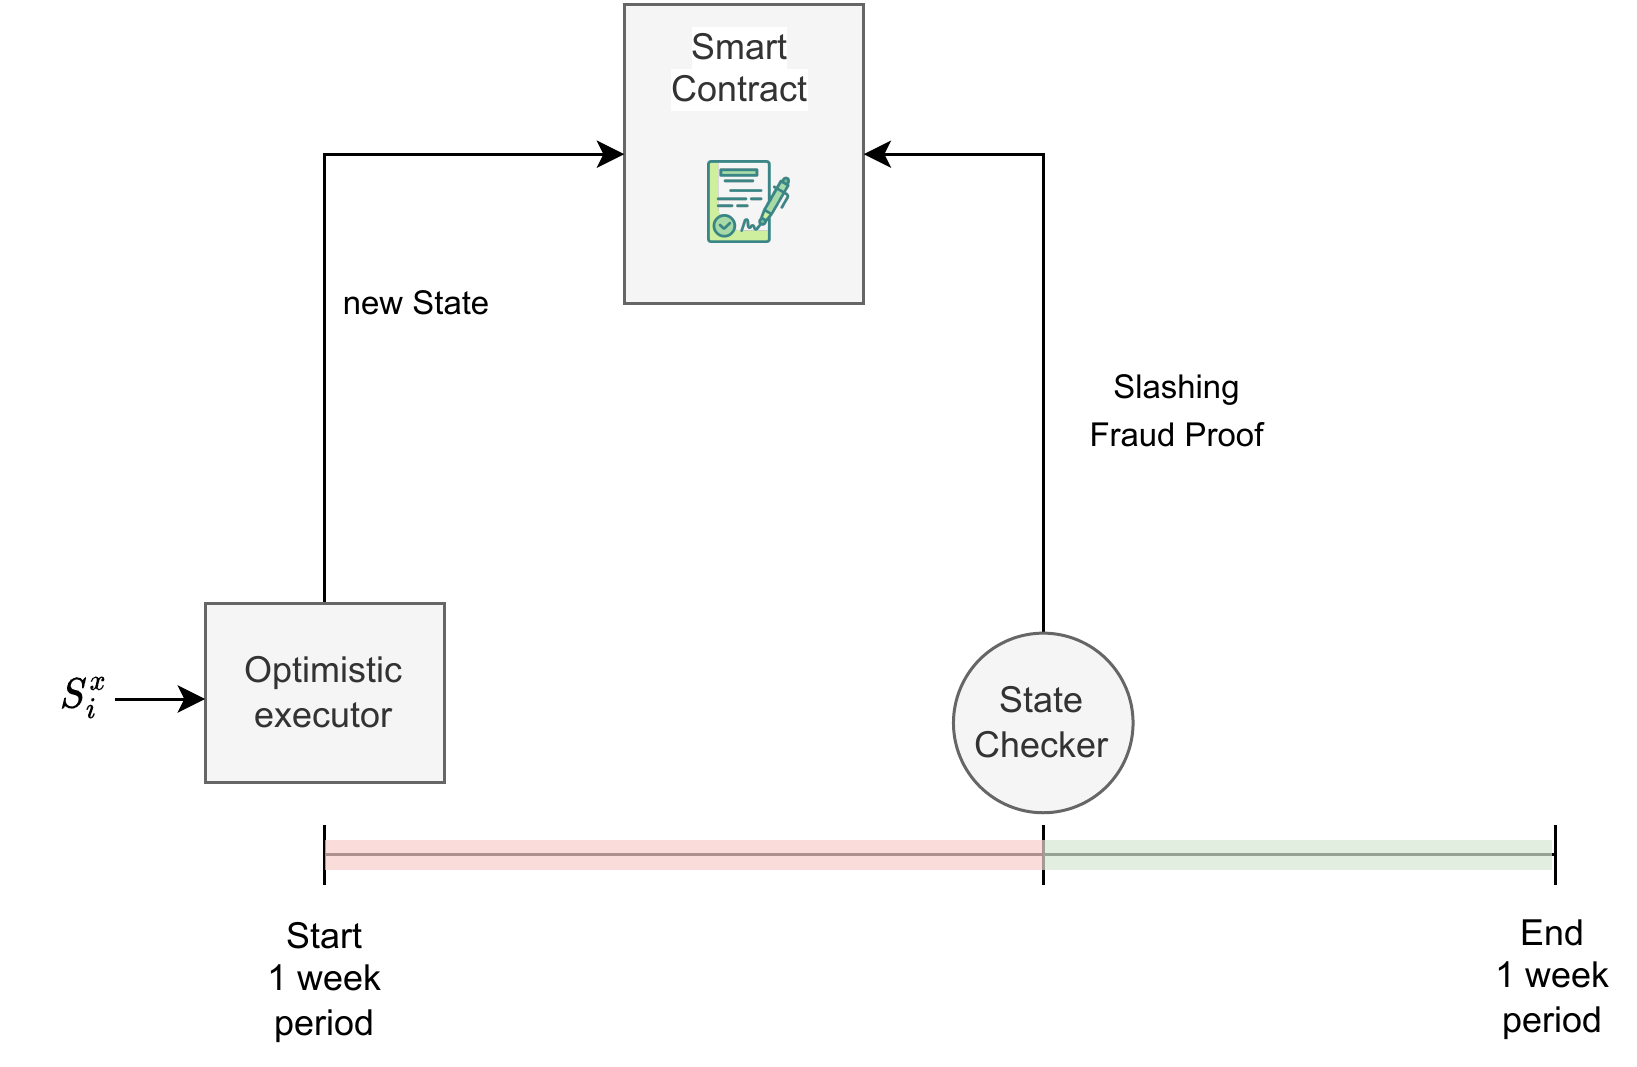
\includegraphics[width=.75\columnwidth]{\trainingsectiondir/figures/optimistic-fraud-proof.drawio}
\caption{Optimistic Execution Schema of a Fraud Proof.}
\label{fig:optimistic-execution}
\end{figure}

\item \textbf{Succinct Computation Verification (Zero-Knowledge Technology)}: The third approach leverages zero-knowledge technology to enable succinct computation verification. In this method, transactions are processed and verified in a manner that allows third parties to efficiently confirm the validity of computations without needing to replicate them. In the succinct execution verification model, instead of an optimistic executor, we have an
execution prover (see Figure \ref{fig:zk-rollup}).

The \textbf{prover} is the entity responsible for generating a proof the new L2 state is correctly computed from the previous state and a given set of L2 transactions (which is called a \textbf{batch}) by using zero-knowledge techniques. The \textbf{verifier} role, which have to confirm the validity of the proofs, is assumed by a smart contract located in the the Layer 1 that is also responsible for storing the set of states. The proof size is exceptionally succinct, consisting of just a few bytes. This compactness reduces data storage and transmission requirements. Verification time is notably brief, typically of the order of microseconds $(\mu s$). This inherent properties of the proof enable a smart contract to perform successful verification.

When the verifier smart contract executes the L1 \texttt{verifyBatch()} transaction, we say that the next state, $S^x_{i+1}$, is \textbf{consolidated}. With this approach, the state computation is quickly considered final since it takes only ``seconds or minutes” to generate and validate the proof, offering enhanced privacy and scalability.

The \textbf{prover} is typically hosted on a cloud service, allowing for a elastic demand of resources and therefore making it easily accessible and scalable. Provers require a significant amount of computational resources, primarily in terms of RAM and CPU capacity, to generate cryptographic proofs.

\begin{figure}[h!]
\centering
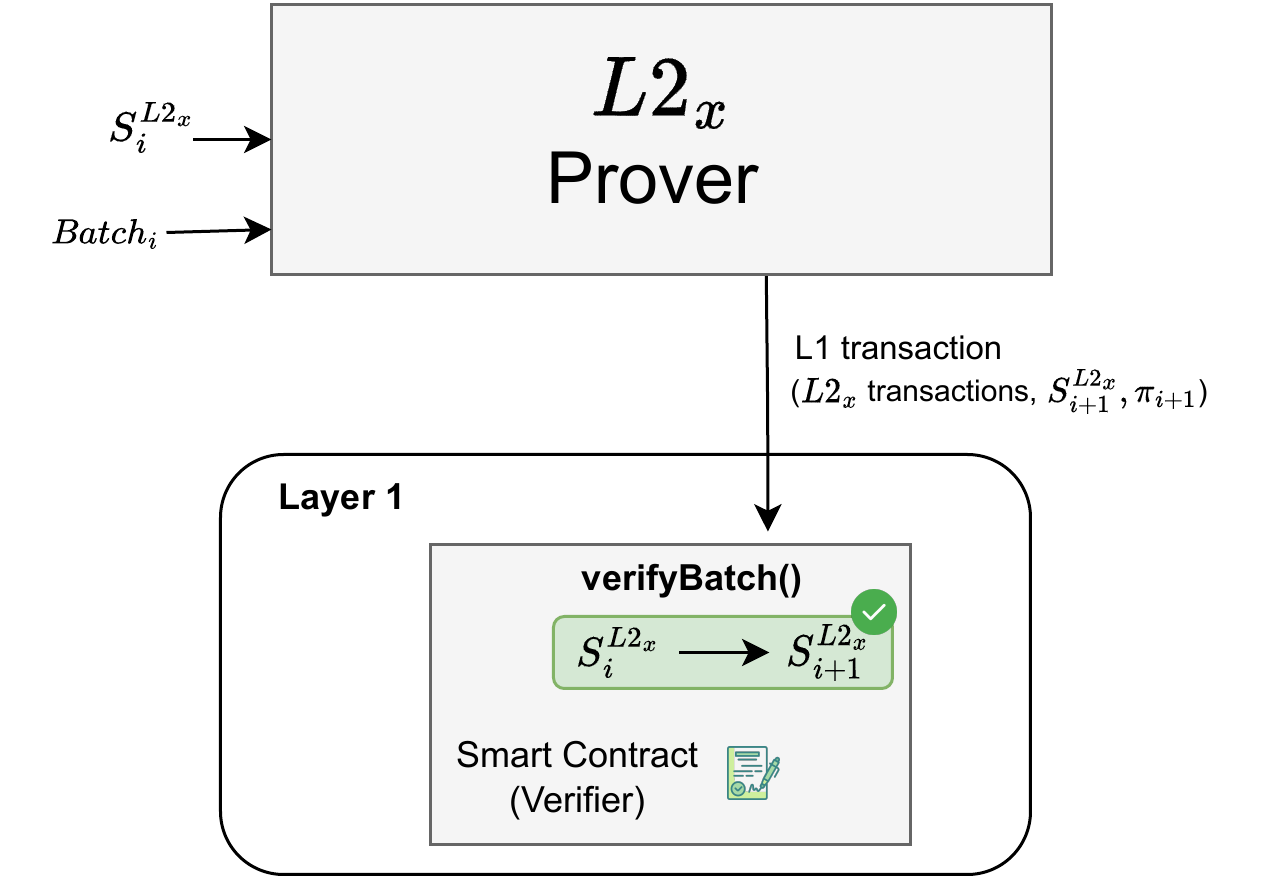
\includegraphics[width=.6\columnwidth]{\trainingsectiondir/figures/succinct-execution-prover-verifier.drawio}
\caption{Succinct Computation Verification Schema.}
\label{fig:zk-rollup}
\end{figure}

However, since all the L2 data is somehow posted in the L1, the natural question that if we are scaling with rollups based on succinct verification arises. The answer is \textbf{yes}, because the smart contract execution resources for verifying a proof are much lower than executing individual transactions within a batch. In fact, the majority of the cost comes from the data availability, but we can work on improve its costs (using succinct verification of compressed data or proto-danksharding when available).

\end{itemize}

It's important to recognize that the choice of method can significantly impact the performance, security, and decentralization characteristics of the L2 ecosystem. Hence, careful consideration and alignment with specific use cases are essential when selecting the appropriate approach.

\subsection{Summary of L2 Scaling Solutions}

Scalability solutions for blockchains can be systematically categorized along two main dimensions:

\begin{itemize}

\item \textbf{Data Availability}: Whether the data from the L2 chain is available on-chain (in L1) or off-chain.

\item \textbf{Mechanism to state correctness}: The methods employed to guarantee the correctness and validity of the L2 chain's state.

\end{itemize}

The table below offer a clear and concise overview of how various solutions align with the criteria of data availability and the mechanism for state correctness.

\begin{figure}[H]
\centering
\begin{tabular}{|c|c|c|}
\hline
\cellcolor{darkgray} & \cellcolor{darkgray} \color{white} Validity Proof  & \cellcolor{darkgray} \color{white} Fraud Proof \\ \hline
\cellcolor{lightgray} Data on-chain   & zkRollup       & Optimistic Rollup \\ \hline
\cellcolor{lightgray} Data off-chain  & zkValidium     & Plasma \\ \hline
\end{tabular}
\end{figure}


One noteworthy feature of the zkValidium approach is its reliance on Zero-Knowledge processing to ensure that even if L2 operators withhold data from users, the cryptographic validation mechanisms guarantee the correct processing of transactions (See Figure \ref{fig:validium-process}). This means that, despite the lack of visibility into individual L2 transactions users can be guaranteed about correctness of the current L2 state. This approach is more cost-effective compared to the zkRollup approach, that consists on writing data directly to the L1 blockchain.

\begin{figure}[h!]
\centering
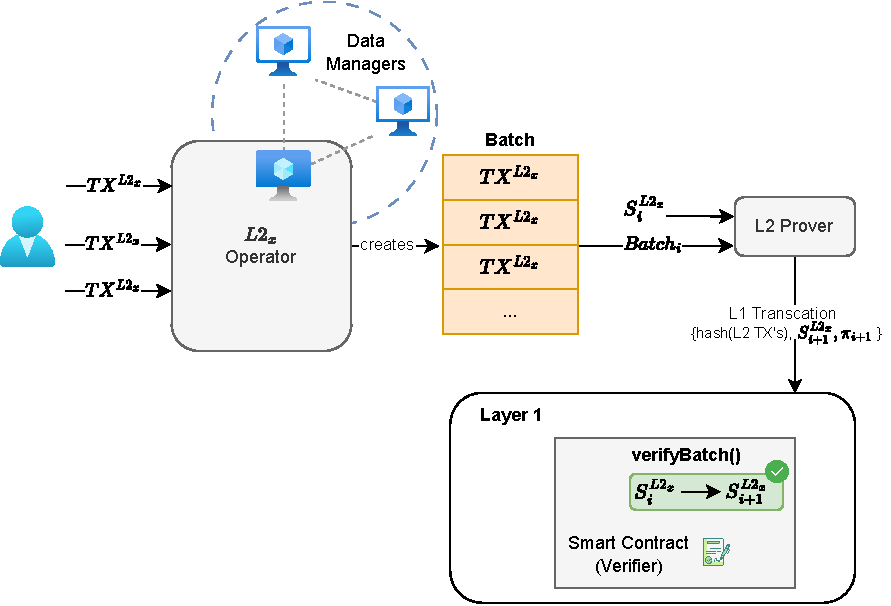
\includegraphics[width=.75\columnwidth]{\trainingsectiondir/figures/validium.drawio}
\caption{zkValidium Batch Verification Process.}
\label{fig:validium-process}
\end{figure}



\subsection{Supported Application Complexity}

Within Layer 2 solutions, the scope of supported functionalities can be categorized into two primary types:

\begin{itemize}

\item \textbf{Simple Processing} (Figure \ref{fig:simple-processing}): This category encompasses solutions that involve the simple transfer of digital assets, such as tokens or payments, with relatively straightforward processing requirements.

\begin{figure}[h!]
\centering
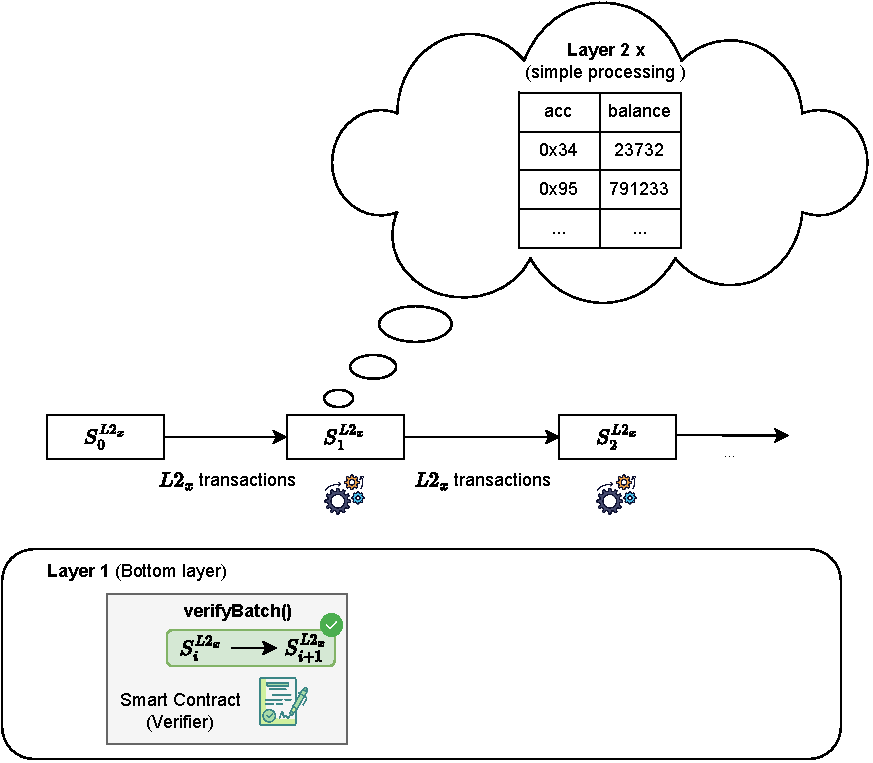
\includegraphics[width=.65\columnwidth]{\trainingsectiondir/figures/l2-simple-processing.drawio}
\caption{Simple Processing Schema.}
\label{fig:simple-processing}
\end{figure}

\item \textbf{General-Purpose Execution Virtual Machine} (Figure \ref{fig:rich-processing}): This category extends the capabilities of L2 solutions to encompass a broader spectrum of functionalities. The hallmark of this category is the utilization of a General-Purpose Virtual Machine, such as the Ethereum Virtual Machine (EVM), enabling ``rich processing" of transactions.

\begin{figure}[h!]
\centering
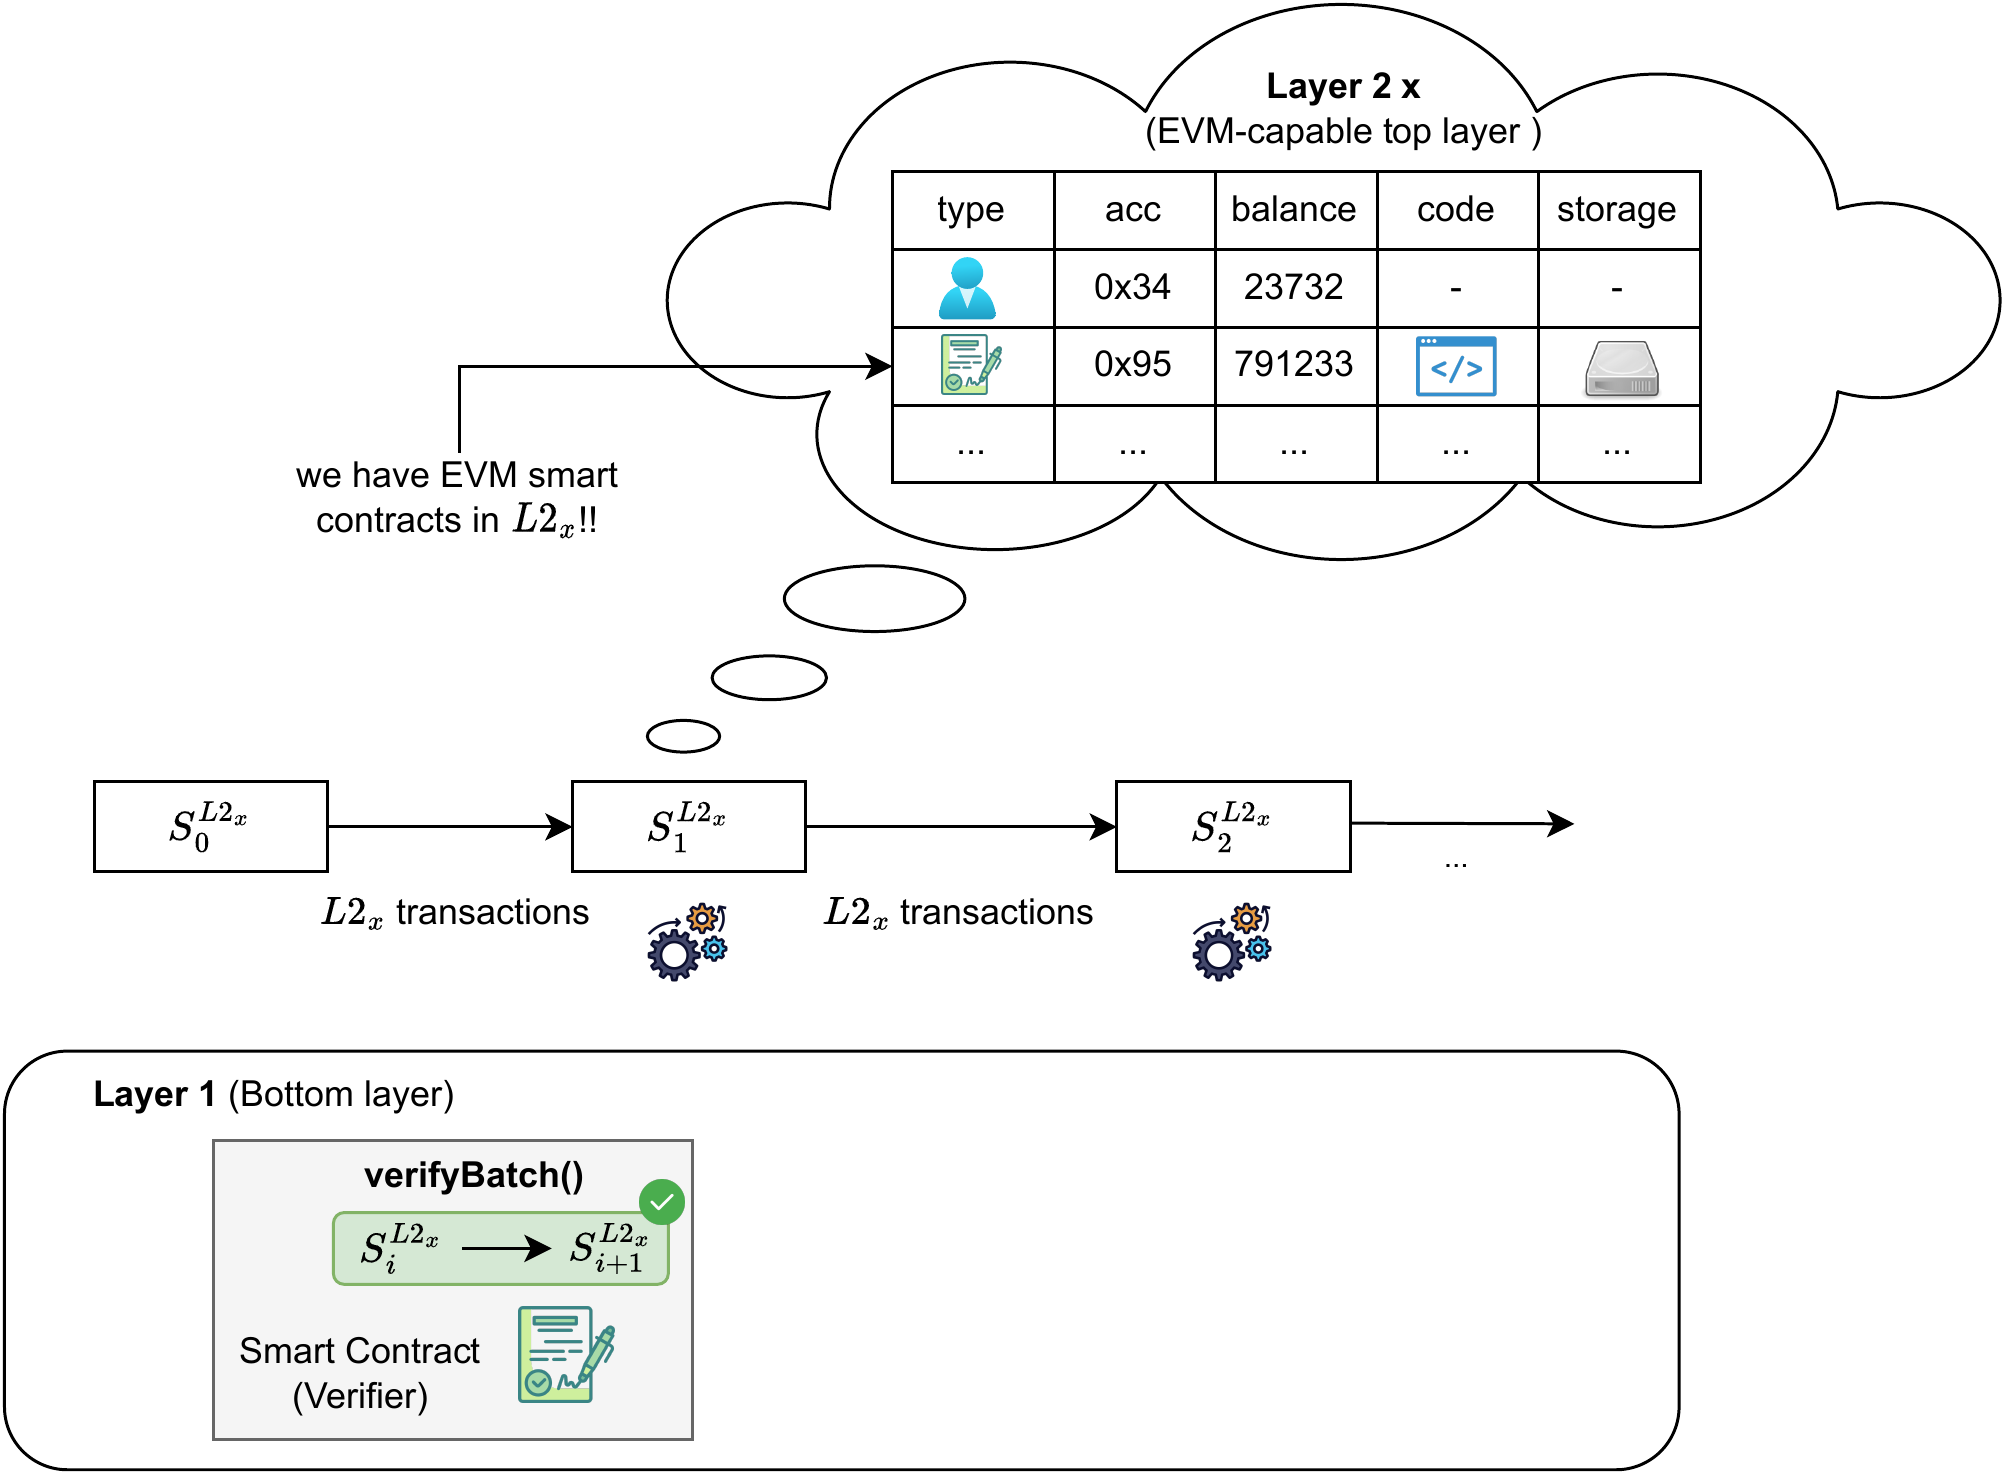
\includegraphics[width=.65\columnwidth]{\trainingsectiondir/figures/l2-rich-processing-zkevm.drawio}
\caption{EVM-like Processing Schema.}
\label{fig:rich-processing}
\end{figure}

\end{itemize}


\subsection{Answering the L2 Design Questions for the Polygon zkEVM}

\begin{itemize}

\item \textbf{How users send L2 transactions and who receives them?}

The zkEVM uses unicast to let user send their transaction (via RPC calls). The zkEVM also enables posting L2 transactions via a method in a smart contract as an anti-censorship measure (called ``forced batches”).

\item \textbf{How L2 transactions are made publicly available (if so)?}

The zkEVM is a rollup, the L2 data is available in L1.

\item \textbf{Who process the L2 transactions and how, and, when it is publicly considered that a new state is correctly computed?}

In the zkEVM, currently, there is a centralized aggregator node that proves the processing of the L2 transactions. However, this node cannot cheat because there is a succinct computation verification (using zero-knowledge technology).

\item \textbf{What type of applications the L2 supports? The processing is simple or rich?}

zkEVM is rich processing since it is an EVM.

\end{itemize}

